\section{Background} \label{sec:Background}

\subsection{Model-driven video game development}
%Video games are pieces of software that, like any other software, need to be designed, developed, and maintained over time. However, there are some particularities of video games that make them differ from traditional software, such as the artistic component of the videogame, the complexity of the rendering pipelines, the heterogeneous nature of video game development teams, and the abstract nature of the final purpose of a video game: fun~\cite{pascarella2018video, chueca2023consolidation}. 
%Hence, video games present characteristics that differentiate their development and maintenance from the development and maintenance of classic software. Examples of these differences can be found in how video game developers must contribute to the implementation of different kinds of artifacts (e.g., shaders, meshes, or prefabs) or in the challenges they face when locating bugs or reusing code~\cite{pascarella2018video, chueca2023consolidation}.
Nowadays, most video games are developed by means of game engines. Game engines are development environments that integrate a graphics engine and a physics engine as well as tools for both to accelerate development. The most popular ones are Unity and Unreal Engine, but it is also possible for a studio to make its own specific engine (e.g., CryEngine~\cite{cryengine}). 

One key artefact of game engines are software models. Unreal proposes its own modeling language (Unreal Blueprints)~\cite{unrealblueprint}, Unity propposes Unity Visual Scripting~\cite{unityscripting}, and a recent survey in Model-Driven Game Development~\cite{zhu2019model} reveals that UML and Domain Specific Language (DSL) models are also being adopted by development teams. Developers can use the software models to create video game content instead of using the traditional coding approach. While code allows for more control over the content, software models raise the abstraction level, thus promoting the use of domain terms and minimizing implementation and technological details. Through software models, developers are freed from a significant part of the implementation details of physics and graphics, and can focus on the content of the game itself (see Figure.~\ref{fig:architecture}).

\begin{figure}[h]
    \centering
    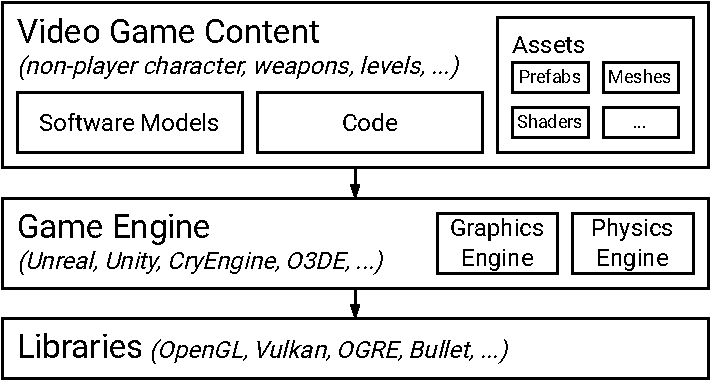
\includegraphics[width=0.35\textwidth]{Figures/fig_bg_OverviewArtifactsVG.pdf}
    \caption{Overview of video game artefacts.}
    \label{fig:architecture}
\end{figure}

\subsection{\CaseStudy{}}
We evaluate our novel proposal for PCT, \ApproachName{} in an industrial case study carried out in collaboration with the developers of the commercial video game \CaseStudy{}. Each level of \CaseStudy{} consists of a three-dimensional space where a player-controlled spaceship has to fly from a starting point to a target destination, reaching the goal before being destroyed. The gameplay experience involves exploring floating structures, avoiding asteroids, and finding items along the route, while basic enemies try to damage the spaceship by firing projectiles. If the player manages to reach the destination, the ultimate antagonist corresponding to that level (which is referred to as \textit{boss}) appears and must be defeated in order to complete the level. \CaseStudy{}'s boss is the NPCs target content that we aim to automatically create via PCT. Bosses can be built either using C++ code or software models. The top part of Figure~\ref{fig:scenario} depicts a boss fight scenario where the player-controlled ship (item A in the figure) is battling the NPC Serpent (item B in the figure), which is the final boss that must be defeated in order to complete Level 1. The bottom part of Figure~\ref{fig:scenario}  illustrates the two possible development approaches for the Serpent boss (model-driven Vs. code-centric).

\begin{figure}[tb]
    \centering
    \includegraphics[width=\columnwidth]{Figures/MM_Scenario.pdf}
    \caption{Model-Driven Development vs. Code-Centric Development in the context of \CaseStudy{}}
    \label{fig:scenario}
\end{figure}

%Even though Figure~\ref{fig:scenario} shows excerpts of the implementation of the Serpent both in the form of software models and code, it is not necessary to realize both in order to implement this content. 
Developers can mix both technologies by developing different parts of the boss using one or the other approach indistinctly, but they are also free to implement the content using software models exclusively or to do so purely via code. However, the heterogeneous nature of video game development teams - comprised majorly of programmers~\cite{devNation}, but also counting game designers, artists, UI designers, and QA engineers within their ranks - possibly favours the use of software models over code thanks to the higher abstraction level of the former (combined with their detachment from more technical implementation details) which empowers less tech-focused roles to embrace a more active participation in development tasks.  Also, previous work~\cite{domingo2020evaluating} showed that video game developers make fewer mistakes and are more efficient when working with models rather than code.

In \CaseStudy{}, the elements of the game are created through software models, and more specifically, through the Shooter Definition Model Language (SDML). SDML is a DSL model for the video game domain that defines aspects that are included in video game entities: the anatomical structure (including their components, physical properties, and connections); the amount and distribution of vulnerable parts, weapons, and defences; and the movement behaviours associated to the whole body or its parts. SDML has concepts such as hulls, links, weak points, weapons, and AI components, and allows for the development of all types of video game content, such as bosses, enemies, or environmental elements. The models are created using SDML and interpreted at runtime to generate the corresponding game entities. In other words, software models created using SDML are translated into C++ objects at runtime using an interpreter integrated into the game engine~\cite{blasco2021evolutionary}. More information on the SDML model can be found on-line at \url{https://youtu.be/Vp3Zt4qXkoY}.